% FEEDBACK
%
% !TEX root = ../thesis-main.tex
%
\chapter{Feedback on lexical stress errors}
\label{chap:feedback}

%\cleanchapterquote{You can’t do better design with a computer, but you can speed up your work enormously.}{Wim Crouwel}{(Graphic designer and typographer)}

 	\citep{Hattie2007}

%TODO replace after proposal
%	\begin{figure}[htb]
%		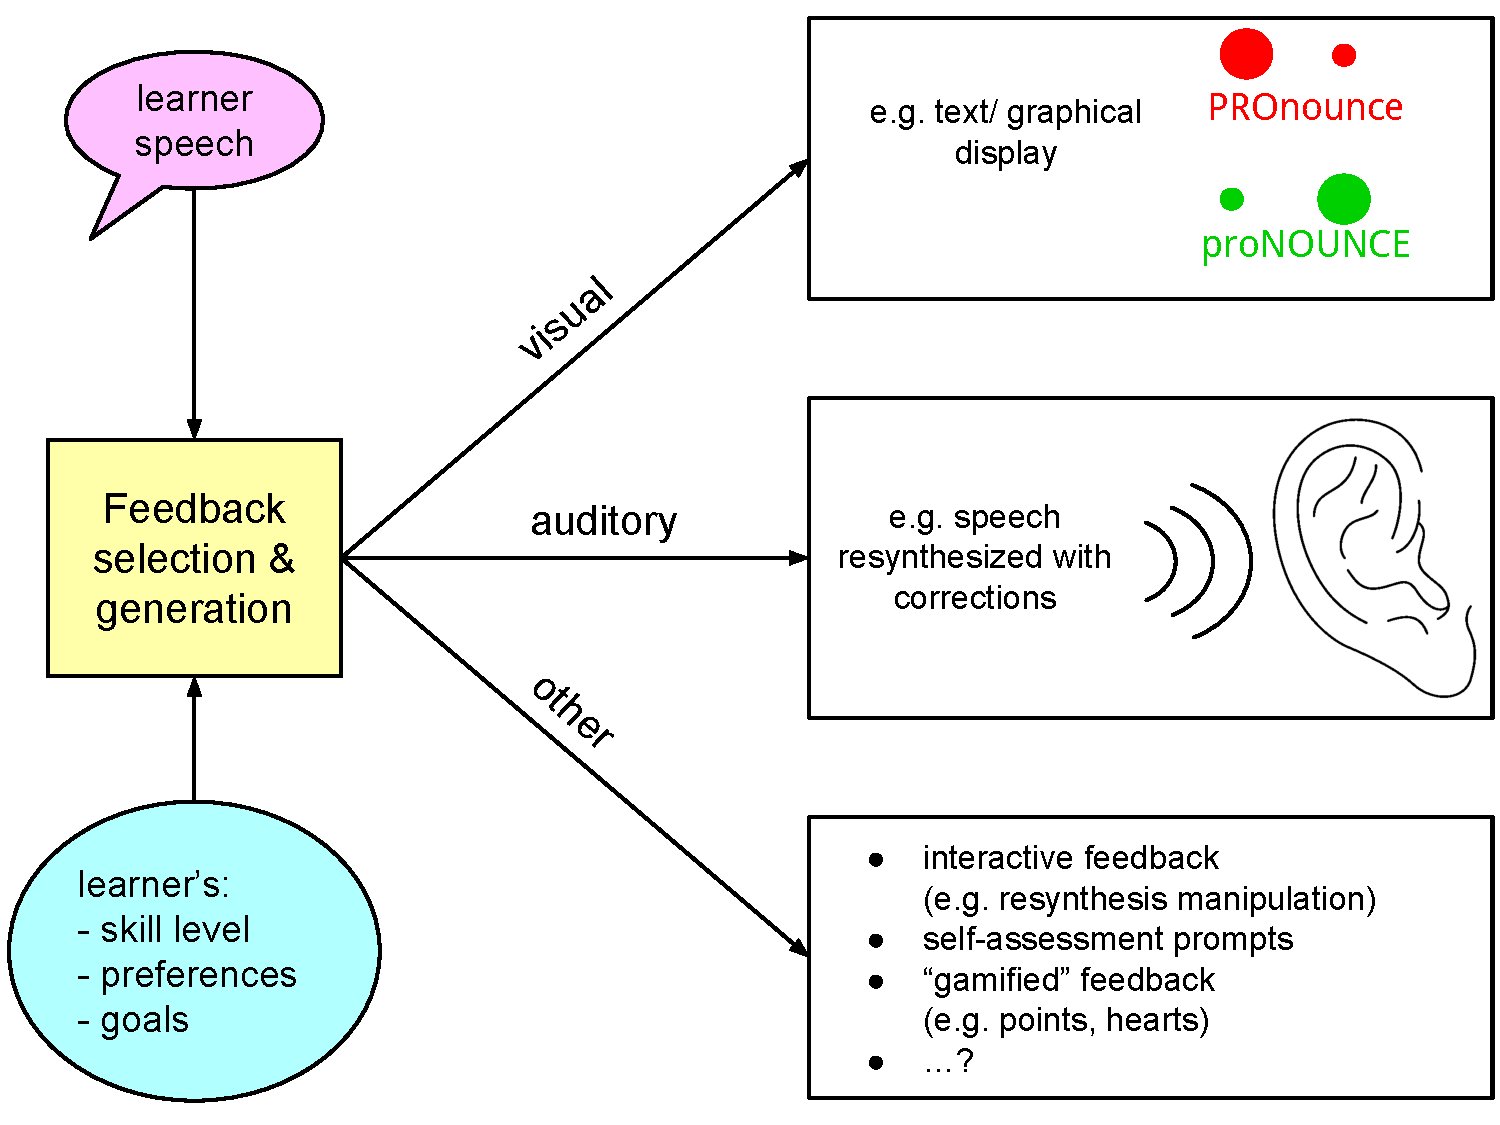
\includegraphics[width=\textwidth]{../img/feedback}
%		\caption{Delivery of prosody feedback in different modalities.}
%		\label{fig:feedback}
%	\end{figure}

%\section{Related work}
%\label{sec:fb:related}
%
%	\cite{Sitaram2011}
%	\cite{Bonneau2011}
%	 	\citep{Hattie2007}


\section{Visual feedback}
\label{sec:fb:visual}

\citep{Sitaram2011}

%TODO replace
%	\subsection{Stylized text}
%	\label{sec:visual:text}
%	
%TODO replace
%	\subsection{Graphical representations of prosody}
%	\label{sec:visual:graphics}
%	
%TODO replace
%	\subsection{Visualizations of the speech signal}
%	\label{sec:visual:visualizations}
	
	
	
\section{Auditory feedback}
\label{sec:fb:auditory}

\citep{Bonneau2011}

%TODO replace
%	\subsection{Enhanced reference utterance}
%	\label{sec:auditory:enhanced}
%	
%TODO replace
%	\subsection{Resynthesized learner speech}
%	\label{sec:auditory:resynth}
	
	
	
\section{Alternative feedback types}
\label{sec:fb:alternative}

%TODO replace
%	\subsection{Metalinguistic feedback}
%	\label{sec:alternative:metaling}
%	
%TODO replace
%	\subsection{Interactive feedback}
%	\label{sec:alternative:interactive}
%	
%TODO replace
%	\subsection{Implicit feedback}
%	\label{sec:alternative:implicit}

\section{Summary}
\label{sec:fb:summary}